%!TEX root = ../thesis.tex

\chapter{Background \& Motivation}
In this chapter, we first motivate the need for stochastic models with a simple example predicting the path of a drifter in the Gulf Stream.o

Throughout, we will use an example of tracking a drifter in the Gulf Stream to illustrate the concepts introduced.
We will return to this example in more detail, including applying our later developments, in \Cref{ch:appls}.

We then briefly review the current literature on stochastic parameterisation, which is the introduction of stochastic terms into otherwise deterministic models, in the context of atmospheric modelling, oceanography and climate forecasting.
Finally, we highlight the limitations of bulk stochastic simulation as a means of working with complicated stochastic models, both in terms of computational costs and accuracy.
This suggests the need, across a variety of applications, for developing computationally efficient methods for approximating prediction distributions of such stochastic models, which this thesis aims to address.


\section{Preliminaries}
\subsection{Notation}
We start this chapter by introducing the mathematical notation that will be used throughout this thesis.

The set of \(n \times m\) matrices with real-valued entries is denoted as \(\R^{n\times m}\).
In general, the \(i\)th component of a vector \(x\) is denoted by \(x_{i}\), except where there is already a subscript, in which case we write \(x_t^{(i)}\) to denote the \(i\)th component of \(x_t\), for instance.
The norm symbol \(\norm{\cdot}\) without any additional qualifiers denotes the standard Euclidean norm for a vector, and the spectral (operator) norm induced by the Euclidean norm, i.e. for an \(n \times n\) matrix \(A\)
\[
	\norm{A} = \sup\left\{\frac{\norm{Av}}{\norm{v}}\,\middle|\,v \in \R^n, \, \norm{v} \neq 0\right\}.
\]


\subsection{Probability theory}
For a random variable \(X\), we use \(\avg{X}\) to denote the expectation of \(X\) and \(\var{X}\) to denote the variance.
For a \(n\)-dimensional vector-valued random variable \(Y\), \(\avg{Y}\) again denotes the (now vector-valued) expectation of \(Y\), and \(\var{Y}\) denotes the covariance matrix of \(Y\).
That is, \(\var{Y}\) is the \(n\times n\) matrix with \((i,j)\)th component
\[
	\left[\var{Y}\right]_{ij} = \avg{Y_iY_j} - \avg{Y_i}\avg{Y_j} = \mathrm{Cov}\left(Y_i, Y_j\right) = \begin{cases}
		\var{Y_i},                         & \text{if } i = j, \\
		\mathrm{Cov}\left(Y_i, Y_j\right), & \text{otherwise}.
	\end{cases}
\]

There are several different notions of convergence for a sequence of random variables, which we briefly recall here.
Consider a sequence of \(m\)-dimensional random vectors \(X_1, X_2,\dotsc\) and an \(m\)-dimensional random vector \(X\).
We say that:
\begin{itemize}
	\item The sequence \(X_1, X_2, \dotsc\) converges \emph{in distribution} to \(X\) if
	      \[
		      \lim_{n\to\infty}F_n\left(x\right) = F(x),
	      \]
	      where \(F_n\) is the cumulative distribution function for \(X_n\) and \(F\) is the cumulative distribution function for \(X\), for every point \(x \in \R^m\) where \(F\) is continuous.
	      If this is the case, we write
	      \[
		      X_n \xlongrightarrow[\text{distribution}]{} X, \quad \text{as } n \to \infty.
	      \]
	      Note that the limiting random vector \(X\) need not be defined on the same probability space as the terms in the sequence \(X_1, X_2, \dotsc\); convergence in distribution is the only notion of convergence for which this is the case.


	\item The sequence \(X_1, X_2, \dotsc\) converges \emph{in probability} to \(X\) if for every \(\delta > 0\)
	      \[
		      \lim_{n\to\infty}P\left(\norm{X_n - X} < \delta\right) = 0,
	      \]
	      in which case we write
	      \[
		      X_n \xlongrightarrow[\text{probability}]{} X, \quad \text{as } n \to \infty.
	      \]

	\item The sequence \(X_1, X_2, \dotsc\) converges \emph{almost surely} to \(X\) if
	      \[
		      P\left(\lim_{n \to \infty}X_n = X\right) = 1,
	      \]
	      in which case we write
	      \[
		      X_n \xlongrightarrow[\text{almost surely}]{} X, \quad \text{as } n \to \infty.
	      \]

	\item For \(r > 0\), the sequence \(X_1, X_2, \dotsc\) converges \emph{in \(r\)th mean} to \(X\) if
	      \[
		      \lim_{n\to\infty}{\avg{\norm{X_n - X}^r}} = 0,
	      \]
	      in which case we write
	      \[
		      X_n \xlongrightarrow[r\text{th mean}]{} X, \quad \text{as } n \to \infty.
	      \]
	      This type of convergence is also known as \emph{\(L_r\)-convergence}, as it corresponds to convergence in the \(L_r\) norm on the probability space on which \(X_1,\dotsc, X_n\) and \(X\) are defined.

\end{itemize}
There are implications between each notion of convergence, with convergence almost surely being the strongest and convergence in distribution the weakest.
These implications are summarised in \Cref{fig:rv_conv_impl}.

\usetikzlibrary{positioning}
\begin{figure}
	\begin{center}
		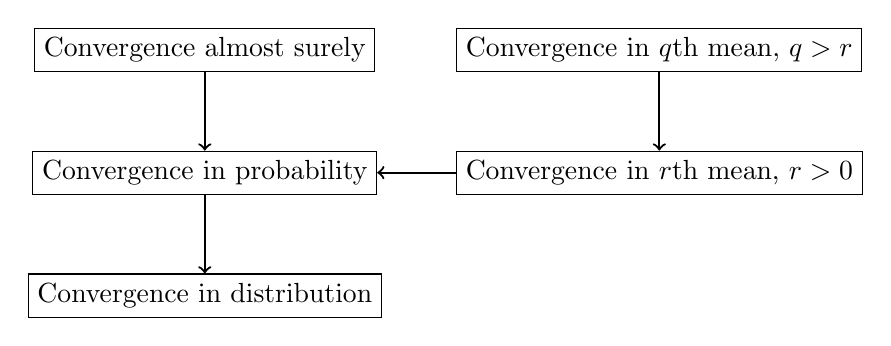
\begin{tikzpicture}
			\node (as) [draw] {Convergence almost surely};
			\node (p) [draw, below=of as] {Convergence in probability};
			\node (rm) [draw, right=of p] {Convergence in \(r\)th mean, \(r > 0\)};
			\node (qm) [draw, above=of rm] {Convergence in \(q\)th mean, \(q > r\)};
			% \node (rmom) [draw, below=of rm] {Convergence of \(r\)th moment};
			\node (d) [draw, below=of p] {Convergence in distribution};
			\path[->,thick] (as) edge  (p)
			(p) edge  (d)
			(qm) edge (rm)
			(rm) edge (p);
			% (rm) edge (rmom);
		\end{tikzpicture}
		\caption{The strength of each notion of convergence in probability, where each directed arrow corresponds to an implication.
			These results are stated and proven in \citet{Bremaud_2020_ProbabilityTheoryStochastic}, for instance.}
		\label{fig:rv_conv_impl}
	\end{center}
\end{figure}







\section{Deterministic dynamical systems}
The continuous time evolution of many different phenomena can be modelled with a system of first order differential equations of the form
\begin{equation}\label{eqn:det_ode}
	\dod{w_t}{t} = u\!\left(w_t, t\right),
\end{equation}
where \(w_t \in \R^n\) is the time-evolving state variable of interest, and \(u \colon \R^n \times [0,T] \to \R^n\) is the vector field.
The governing vector field \(u\) may be specified using existing phenomenological models, but in modern applications these are usually supplemented or driven by observed data~\citep{LawEtAl_2015_DataAssimilationMathematical,ReichCotter_2015_ProbabilisticForecastingBayesian}.
Standard examples include the modelling of weather using available data~\citep{LawEtAl_2015_DataAssimilationMathematical,ReichCotter_2015_ProbabilisticForecastingBayesian}, and predicting concentrations of, for instance, temperature, pollutants or phytoplankton in the ocean using observed current velocity data~\citep{AbascalEtAl_2009_ApplicationHFRadar,dOvidioEtAl_2010_FluidDynamicalNiches}.


We can solve \cref{eqn:ode_det} analytically, or, as is often required in practice, numerically to generate time evolving trajectories, which can inform future predictions or be used to reconstruct past behaviour.

Differential equations of the form \eqref{eqn:det_ode} define a continuous-time dynamical system, and are well-studied.
The flow map of \cref{eqn:det_ode} provides a convenient way of summarising and working with the trajectories that solve \cref{eqn:det_ode}.
Formally, the flow map \(F_{s}^{t}: \R^n \to \R^n\) from time \(s\) to \(t\) associated with \cref{eqn:det_ode} is the unique solution to
\begin{equation}
	\dpd{F_{s}^{\tau}(x)}{\tau} = u\left(F_{s}^\tau(x), \tau\right), \qquad F_{s}^{s}(x) = x,
	\label{eqn:flow_map_ode}
\end{equation}
solved up to time \(\tau = t\).
That is, the flow map is the operator mapping initial conditions at time \(t\) to their corresponding positions at time \(s\), under the continuous-time evolution of \cref{eqn:det_ode}.
% The flow map satisfies several useful properties:
% \begin{itemize}
% 	\item

% 	\item For any \(r \leq s \leq t\),
% 	      \[
% 		      F_r^t\!\left(x\right) = F_s^t\!\left(F_r^s\!\left(x\right)\right).
% 	      \]
% 	      That is,
% 	      This property is illustrated in \Cref{fig:flow_map_diag}.
% \end{itemize}

% \begin{figure}
% 	\begin{center}
% 		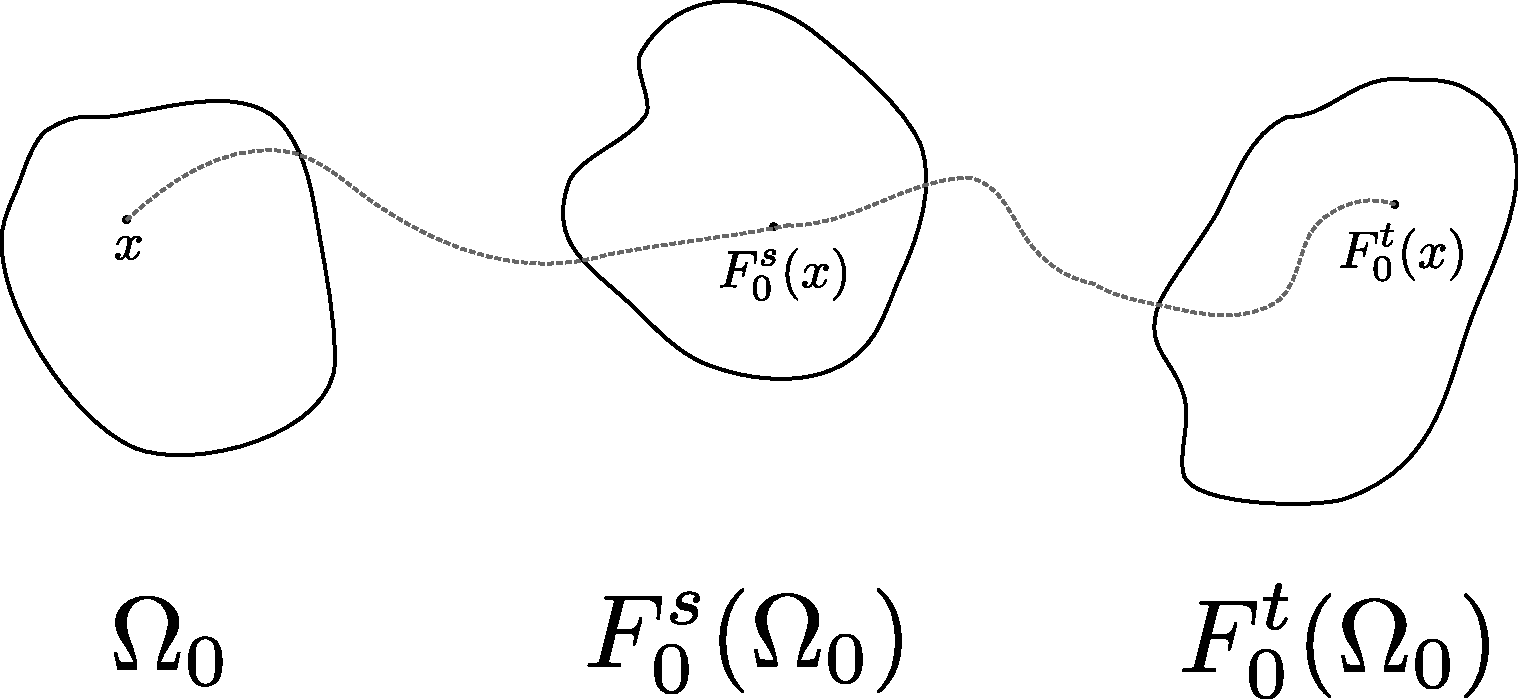
\includegraphics[width=\textwidth]{chp02_background/figures/flow_map.pdf}
% 		\caption{A pictorial representation of the flow map \(F\) corresponding to a continuous time dynamical system.
% 			An initial state \(x\) at time \(0\) is mapped to ..., illustrating the property \(F_s^t\!\left(F_0^s\!\left(x\right)\right) = F_0^t\!\left(x\right)\).}
% 		\label{fig:flow_map_diag}
% 	\end{center}
% \end{figure}


We use the flow map \(F\) to represent all solutions of the deterministic differential equation \cref{eqn:det_ode}, with the understanding that for any relevant initial condition, the flow map at that point can be readily computed by solving the ODE either analytically or numerically.

Moreover, the gradient of the flow map \(F\) (with respect to the initial condition) provides insight into the local behaviour of the dynamical system \citep{Arnold_1973_OrdinaryDifferentialEquations,TruesdellNoll_2004_NonLinearFieldTheories}.
For any times \(s, t \in [0,T]\), this gradient	\(\nabla F_s^t\) satisfies a useful property; the equation of variations.
\begin{equation}
	\dpd{\nabla F_{s}^{t}\!\left(x\right)}{t} = \nabla u\!\left(F_{s}^{t}\!\left(x\right), t\right) \nabla F_{s}^{t}\!\left(x\right).
	\label{eqn:eqn_of_variations}
\end{equation}
This result can be shown by taking the gradient of both sides in \eqref{eqn:flow_map_ode} and using the chain rule.







\subsection{Lagrangian coherent structures}
In this section, we have a brief sojourn into the field of Lagrangian coherent structures, which provide qualitative insight into the behaviour of a dynamical system, particularly in the fluid flow context.

In a steady system (that is, the vector field \(u\) in \cref{eqn:det_ode} is independent of time), we can gain this insight by using classical methods in dynamical systems, such as phase portrait analysis and identifying unstable and stable manifolds.
For example, unstable and stable manifolds cannot be intersected by solution trajectories, and so can act as barriers for the transport of material within a flow.
However, when the system is non-autonomous (that is, the vector field explicitly depends on time \(t\)), these structures can themselves vary with time and the problem of identifying them is far more non-trivial.
Lagrangian coherent structure (LCS) theory provides a mathematical framework for defining and identifying such structures within a given flow \citep{BalasuriyaEtAl_2018_GeneralizedLagrangianCoherent}.


\Cref{fig:lcs_examples} show examples of coherent structures in observed fluid flows, which can be considered LCSs.\lb{Get a proper reference. Photoplankton: \url{https://climate.nasa.gov/climate_resources/170/summer-blooms-in-the-baltic/}}

\begin{figure}
	\begin{center}
		\begin{subfigure}{0.49\textwidth}
			\caption{An oil slick from the \emph{Deepwater Horizon} oil spill in 2010.}
		\end{subfigure}
		\begin{subfigure}{0.49\textwidth}
			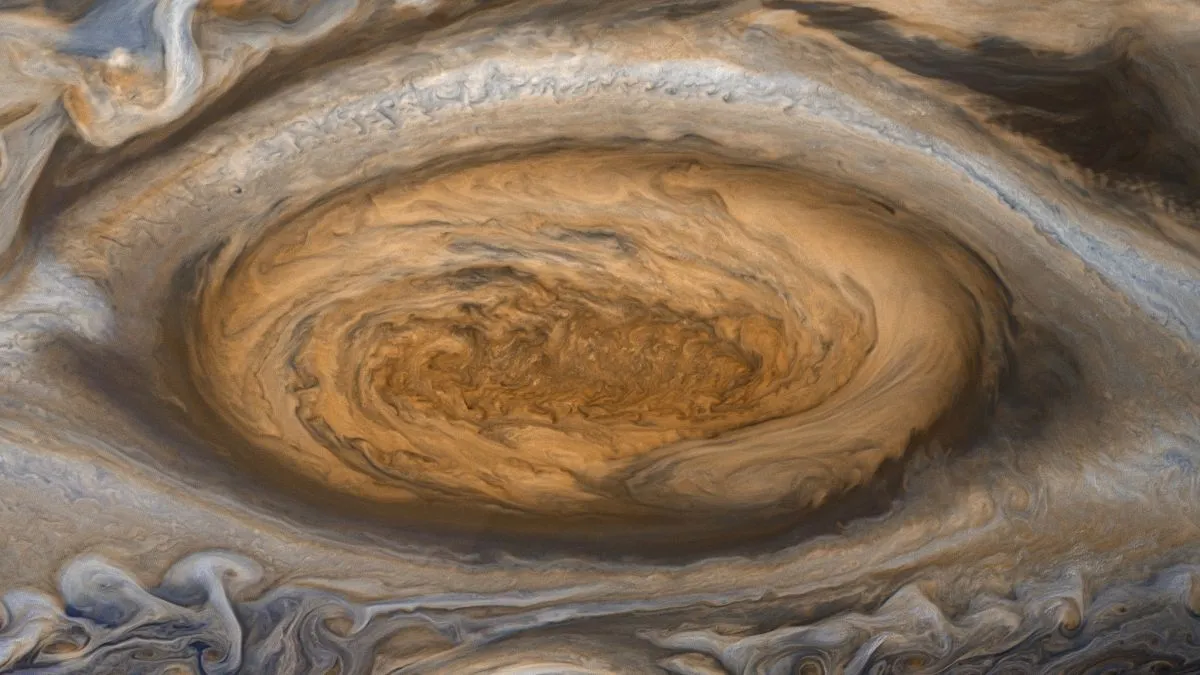
\includegraphics[width=\textwidth]{chp02_background/figures/red_spot.png}
			\caption{Jupiter's Great Red Spot, as photographed by the Voyager probe in 1979 (NASA/JPL-Caltech).}
		\end{subfigure}
		\begin{subfigure}{0.49\textwidth}
			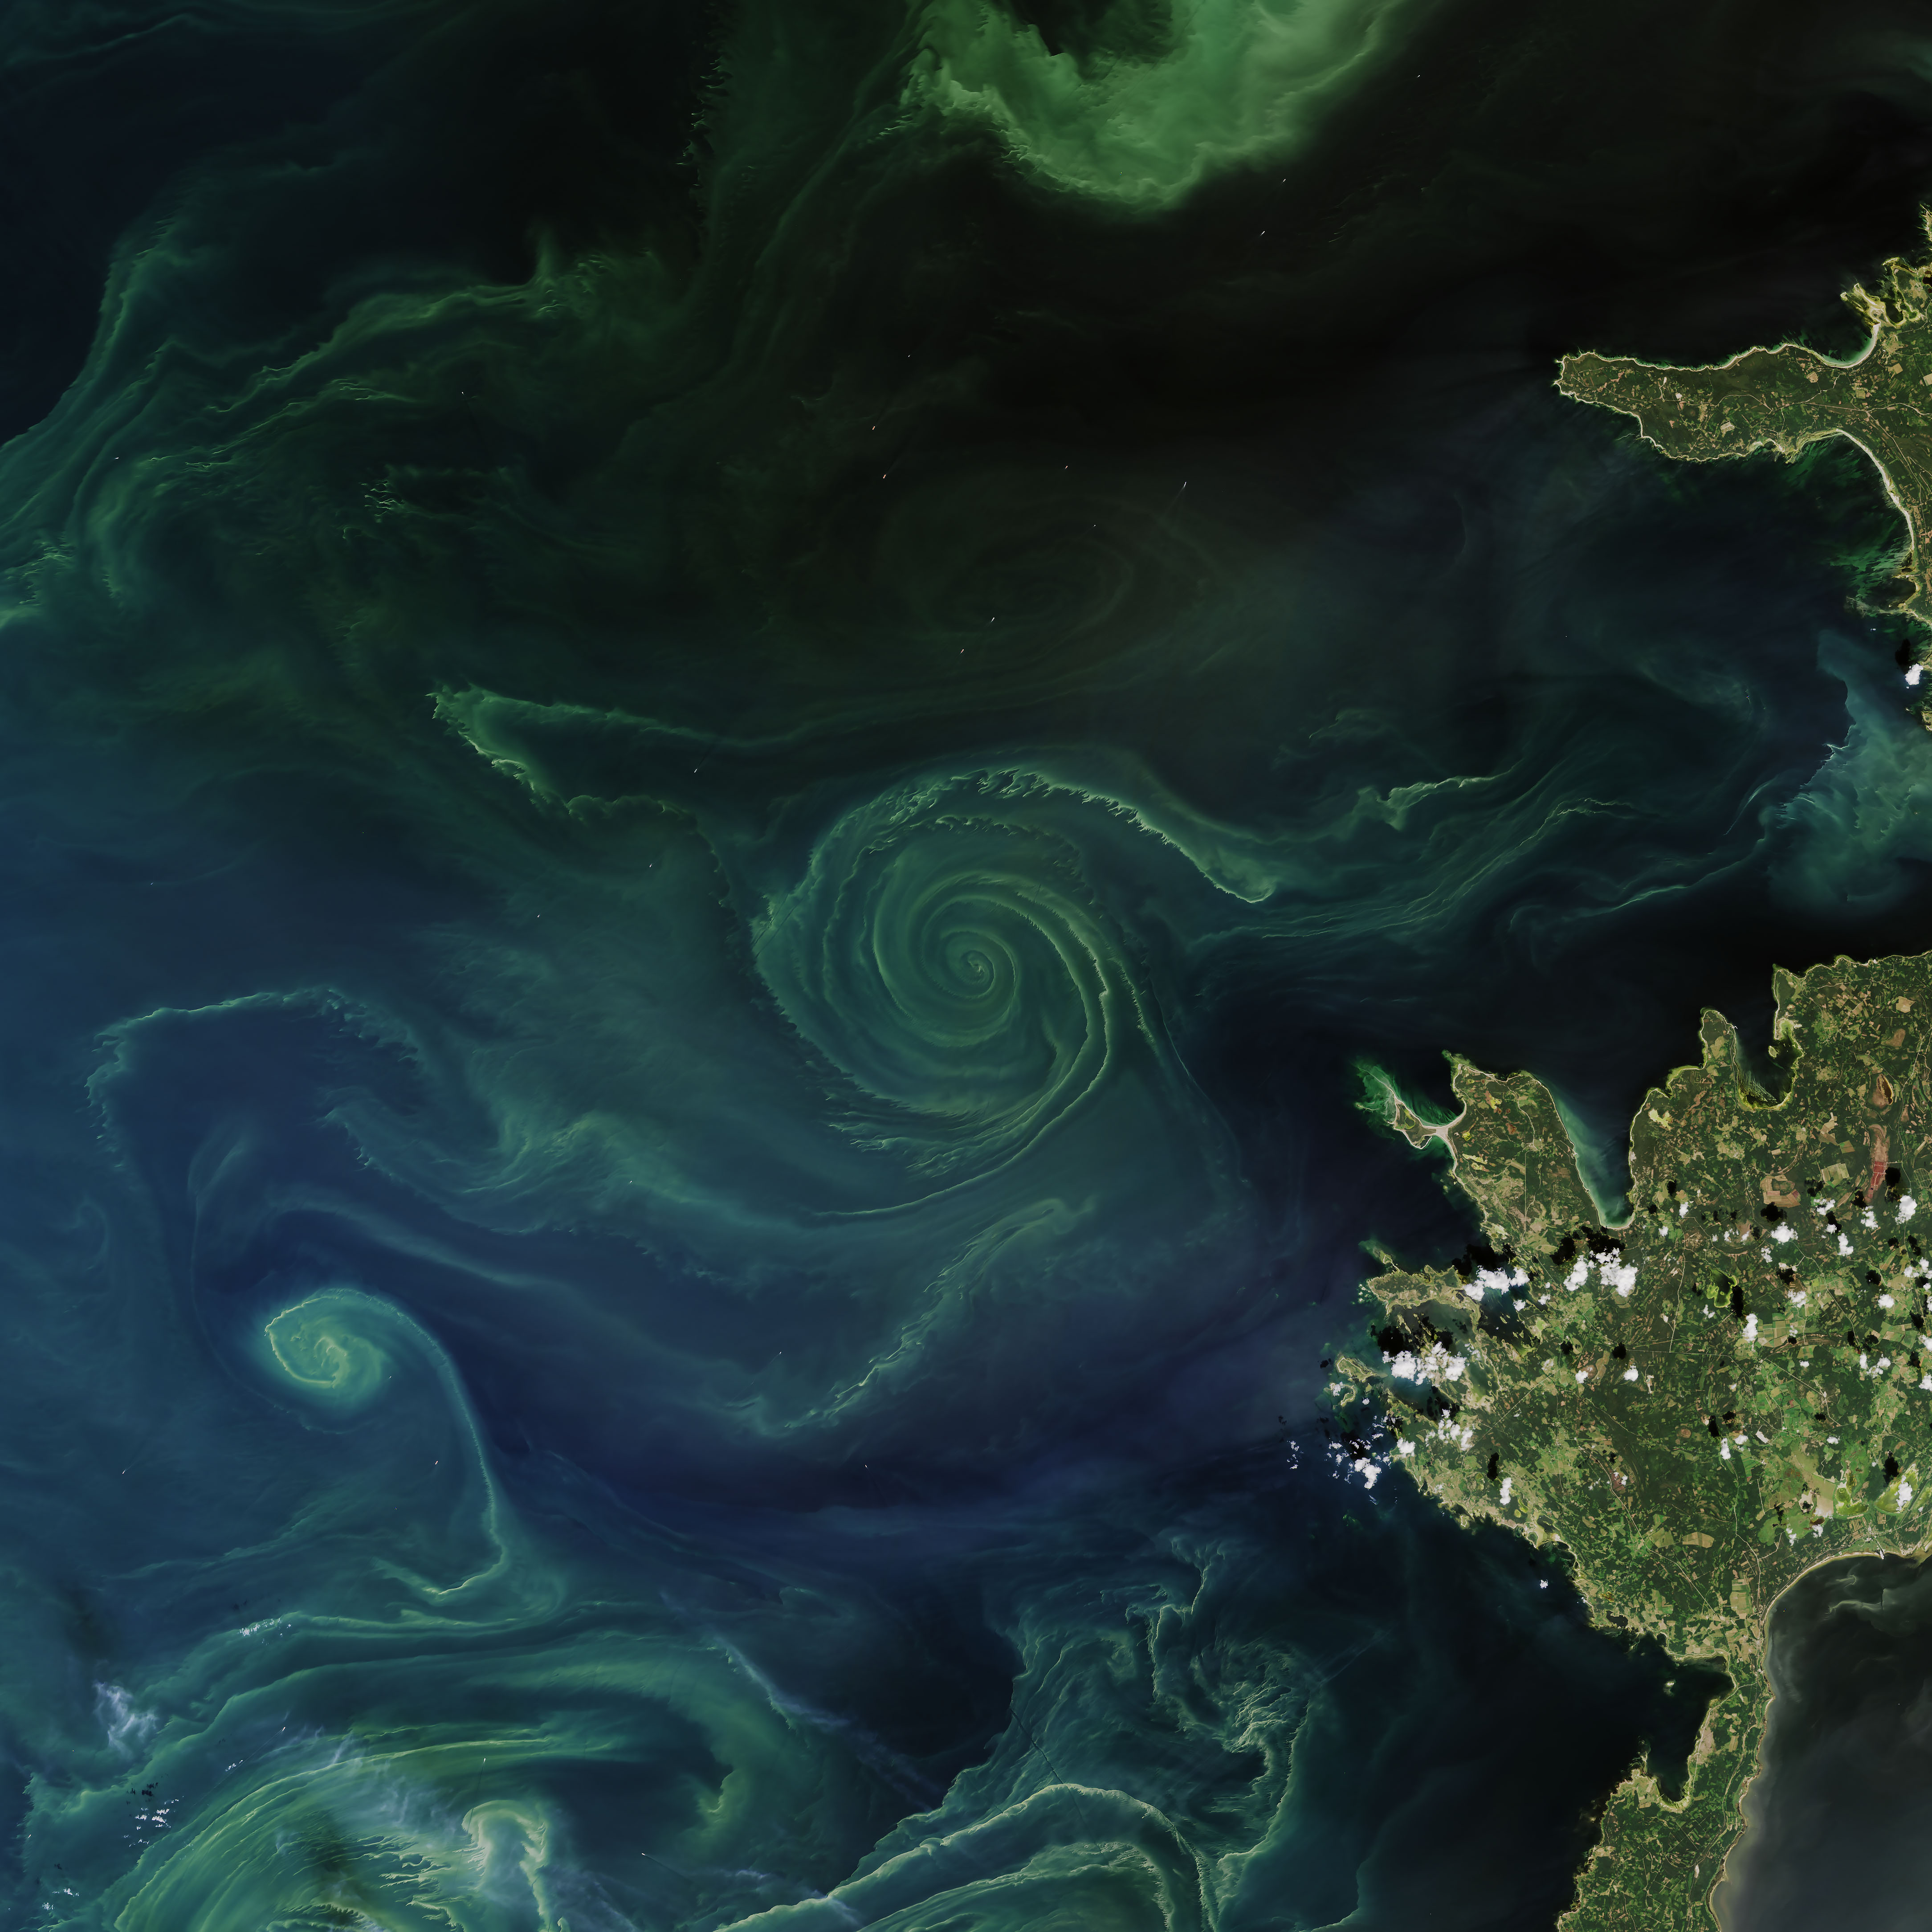
\includegraphics[width=\textwidth]{chp02_background/figures/photoplankton}
			\caption{Photoplankton blooms in the Baltic sea.}
		\end{subfigure}

		\caption{Examples of coherent patterns emerging in fluid flows.}
		\label{fig:lcs_examples}
	\end{center}
\end{figure}


There are many procedures and heuristics for extracting these regions from a given flow, which draw upon
Detailed reviews of approaches to Lagrangian coherent structure extraction are provided by \citet{BalasuriyaEtAl_2018_GeneralizedLagrangianCoherent}, \citet{HadjighasemEtAl_2017_CriticalComparisonLagrangian}, and \citet{PeacockDabiri_2010_IntroductionFocusIssue}, for instance.

One of the best known procedures for extracting LCSs is via the finite-time Lyapunov exponent (FTLE) \citep{ShaddenEtAl_2005_DefinitionPropertiesLagrangian}, which is a measure quantifying the stretching of infinitesimal regions of a flow.


Take an initial condition \(x\) and let \(F_0^t\) represent the flow map of our dynamical system.
We wish to quantify the impact of a small change in the initial condition, so take \(\delta\) as a small and arbitrary perturbation to \(x\).
Then, we measure the \emph{stretching} in the direction of \(\delta\) with
\[
	s\!\left(x, \delta\right) = \frac{\norm{F_0^t\!\left(x + \delta\right) - F_0^t\!\left(x\right)}}{\norm{\delta}}
\]
For sufficiently small \(\delta\), we can replace the mapped perturbation with a linearisation of the flow map about \(x\), that is
\[
	s\!\left(x, \delta\right) \approx \frac{\norm{\nabla F_0^t\!\left(x\right) \delta}}{\norm{\delta}}.
\]
\Cref{fig:ftle_illustr} provides a pictorial representation of this calculation; a small !!!!!
Taking the supremum over all possible perturbations \(\delta\), we have
\[
	\sup_{\delta \in \R^n, \, \delta \neq 0}s\!\left(x, \delta\right) \approx \norm{\nabla F_0^t\!\left(x\right)},
\]
which quantifies the stretching about the trajectory \(F_0^t\!\left(x\right)\).
The finite-time Lyapunov exponent is then computed as
\begin{equation}
	\mathrm{FTLE}_0^t\!\left(x\right) = \frac{1}{\abs{t}}\ln\!\left(\norm{\nabla F_0^t\!\left(x\right)}\right).
	\label{eqn:ftle_defn}
\end{equation}
Note that the operator norm \(\norm{\nabla F_0^t\!\left(x\right)}\) in \cref{eqn:ftle_defn} can be readily computed as the square root of the largest eigenvalue of the Cauchy-Green tensor \(\left[\nabla F_0^t\!\left(x\right)\right]^{\T}\nabla F_0^t\!\left(x\right)\).

% In \Cref{fig:gs_lcs}, we compute the FTLE field of our Gulf Stream velocity model over a timespan of 7 days.



% \begin{figure}
% 	\begin{center}
% 		\begin{subfigure}{0.49\textwidth}
% 			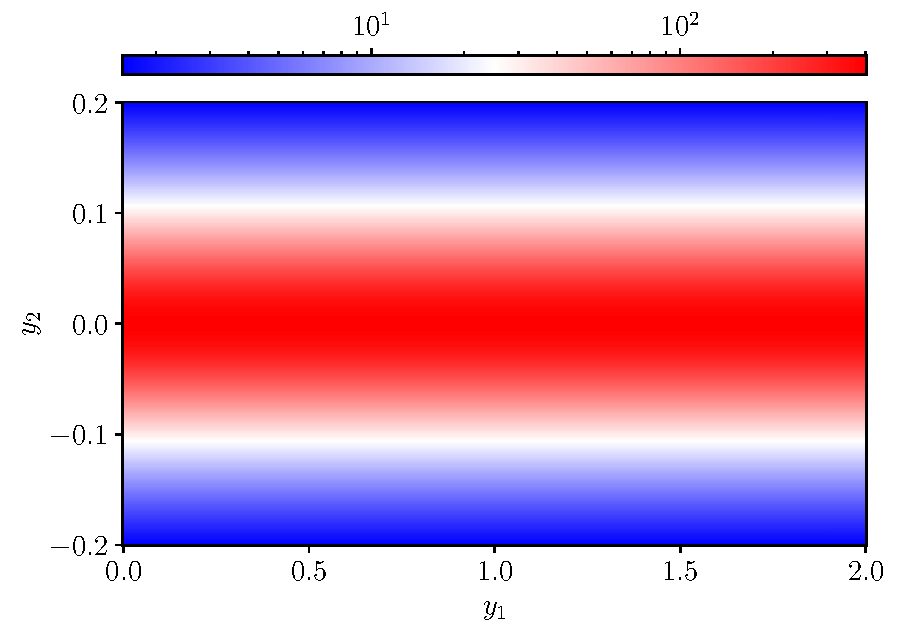
\includegraphics[width=\textwidth]{chp02_background/figures/gulf_stream_motivation/ftle.pdf}
% 			\caption{The finite-time Lyapunov exponent field.}
% 		\end{subfigure}
% 		\begin{subfigure}{0.49\textwidth}
% 			\caption{Maximising ridges of the FTLE field.}
% 		\end{subfigure}
% 		\caption{The finite-time Lyapunov exponent field computed, and corresponding maximising ridges.
% 			This is an example of using a scalar field to extract Lagrangian coherent structures from a fluid flow.
% 			The resulting maximises ridges indicate a skeleton of the Gulf Stream.}
% 		\label{fig:gs_lcs}
% 	\end{center}
% \end{figure}


Most well-established LCS frameworks and extraction procedures are purely deterministic, in that they are defined and compute solely in terms of the dynamical system.
However, uncertainty in such dynamical systems is inevitable and these methods do not explicitly account for this.
There is therefore an emerging interest \citep{Balasuriya_2020_StochasticApproachesLagrangian} in extending LCS theory to stochastic settings (which is the relevance of LCSs to this thesis).
There are several different ways in which stochasticity is being accounted for in LCS frameworks:
\begin{romanate}
	\item in creating novel computable measures that explicitly account for such ongoing uncertainty, e.g. see stochastic sensitivity introduced by \citet{Balasuriya_2020_StochasticSensitivityComputable}, model sensitivity introduced by \citet{KaszasHaller_2020_UniversalUpperEstimate}, and the finite-time divergence rate by \citet{BranickiUda_2023_PathBasedDivergenceRates}.
	These are scalar fields defined on initial conditions that measure, and can be used to extract coherent regions in similar ways to deterministic methods.

	\item \citet{BalasuriyaGottwald_2018_EstimatingStableUnstable} consider stationary flows subject to small-scale stochastic perturbations, and quantify the behaviour of particles
	\citet{DennerEtAl_2016_ComputingCoherentSets} directly compute coherent sets by working with a discretised Fokker-Planck equation.

	\item in understanding the direct impact of velocity uncertainty on well-established deterministic LCS measures.
	\citet{BadzaEtAl_2023_HowSensitiveAre} provide a systematic analysis, using Monte Carlo simulation and summary statistics to evaluate the robustness of several common LCS extraction schemes to velocity uncertainty.
	It is shown that LCS methods that directly account for this uncertainty, such as stochastic sensitivity \citep{Balasuriya_2020_StochasticSensitivityComputable}, are the most robust.
	The finite-time Lyapunov exponent has received particular attention, with an initial study into the impac


\end{romanate}
In this thesis, we are primarily interested point (i), by exploring how our characterisations of uncertainty can be applied to extract coherent structures.
This is directly extending the stochastic sensitivity of \citet{Balasuriya_2020_StochasticSensitivityComputable}, which is summarised in \Cref{sec:s2_summ}.



\section{From ODEs to SDEs}
In practice, any differential equation model will be subject to unavoidable uncertainty, which can arise from a range of sources including but not limited to:
\begin{itemize}
	\item observational errors in any measured data used to construct the model,
	\item uncertainty in any parameters involved in the model,
	\item unexplainable phenomena not captured by the model,
	\item numerical errors in the discretisation of the model, and
	\item uncertainty in the knowledge of the initial state.
\end{itemize}

Since the true nature of this uncertainty is unknowable, it is common to model it as a random process.
That is, we extend our deterministic model to a stochastic one, where the solution (and therefore our predictions of the future state) is now a random variable.
There are several approaches to establishing such a framework, the most general of which is a random dynamical system \citep{Arnold_1998_RandomDynamicalSystems,NeckelRupp_2013_RandomDifferentialEquations}.
However, when working in a continuous-time and continuous-state modelling scenario, a natural extension of an ordinary differential equation to account for this uncertainty is a stochastic differential equation (SDE).
For a formal introduction to stochastic differential equations, see \citet{Oksendal_2003_StochasticDifferentialEquations} or \citet{KallianpurSundar_2014_StochasticAnalysisDiffusion}, for instance.
The following motivation of stochastic differential equations follows a similar one available in \citet{Oksendal_2003_StochasticDifferentialEquations}.

Suppose that we have a deterministic ordinary differential equation, i.e. \cref{eqn:ode_det}, and aim to account for uncertainty in the vector field \(u\).
In lieu of any additional understanding of this uncertainty, we model it as a stochastic noise.
Ideally, we would parameterise the uncertainty with some continuous-time stochastic process \(\xi_t\!\left(x_t\right)\), and write
\[
	\dod{y_t}{t} = u\left(x_t, t\right) + \xi_t\!\left(x_t\right).
\]
The noise process \(\xi_t\) can depend on the state, since we may expect that the magnitude and structure of the uncertainty varies with both the state and time.


Additionally, since we are modelling with a continuum, the noise process \(\xi_t\) should be (with probability \(1\)) continuous in time.
However, such a noise process \(\xi_t\) does not exist \citep{Oksendal_2003_StochasticDifferentialEquations}, in that there is no continuous process with properties 1 to 4, so we need an alternative formulation of the integral.
This leads to the It\^o integral, and It\^o stochastic differential equations, which we introduce in \Cref{sec:bkg_ito} and \Cref{sec:bkg_sde} respectively.



\subsection{The Wiener process}

The Wiener process, or Brownian motion, is an example of a continuous-time stochastic process that is often used to model \td{something}
In the absence of any additional knowledge about the nature of the noise (such as skew)
Defined formally, the (one-dimensional) \emph{Wiener process} is a stochastic process \(B_t\) taking values in \(\R\) and satisfying the following properties:
\begin{romanate}
	\item \(B_0 = 0\),
	\item for every \(s > 0\), the increments \(B_{s + t} - B_{s}\) for \(t \geq 0\) are independent of \(B_r\) for all \(r < s\),
	\item \(B_{s + t} - B_t \isGauss{0, s}\) for all \(s,t > 0\), and
	\item \(B_t\) is continuous in \(t\) almost surely.
\end{romanate}
Remarkably, these properties \emph{uniquely} define the Wiener process, with the additional result that for any \(t > 0\), \(B_t \sim \mathcal{N}\left(0, t\right)\), a Gaussian distribution with mean zero and variance \(t\).
The \emph{\(n\)-dimensional Wiener process} is a stochastic process \(W_t\) taking values in \(R^n\) such that each component of \(W_t\) is a one-dimensional Wiener process and the components of \(W_t\) are mutually independent.
It follows that for the \(n\)-dimensional Wiener process \(W_t\), at any time \(t > 0\), \(W_t \sim \mathcal{N}\left(0, tI\right)\), an \(n\)-dimensional Gaussian distribution with mean zero and covariance matrix \(tI\).

% A Wiener process is a type of L\'evy process, which is a more general class of stochastic process satisfying only conditions (i), (ii), and (iii) above \citep{Applebaum_2004_LevyProcessesStochastic}.

\Cref{fig:wiener_rels} plots realisations of a one-dimensional and two-dimensional Wiener process.

\begin{figure}
	\begin{center}
		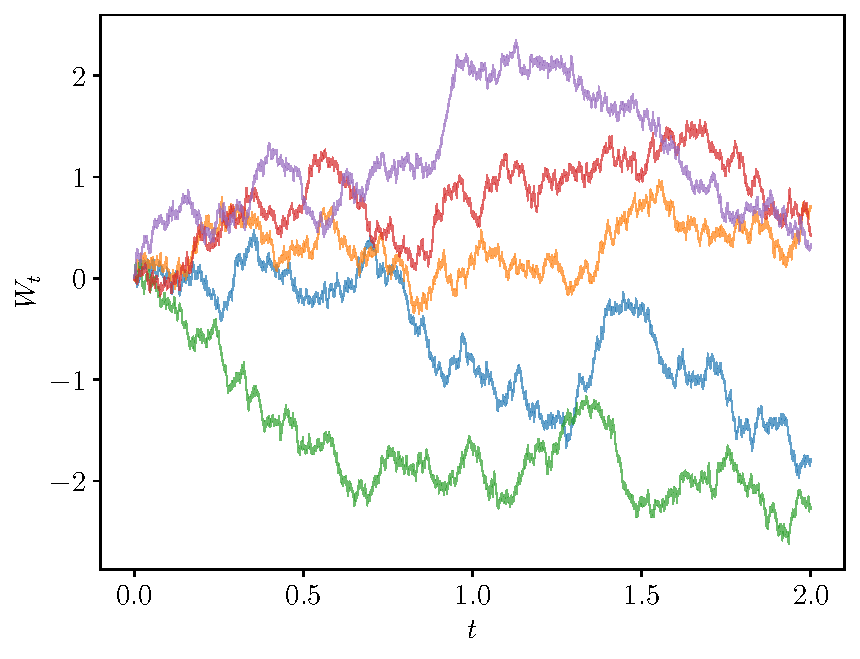
\includegraphics[width=0.49\textwidth]{figures/wiener_realisations_1d.pdf}
		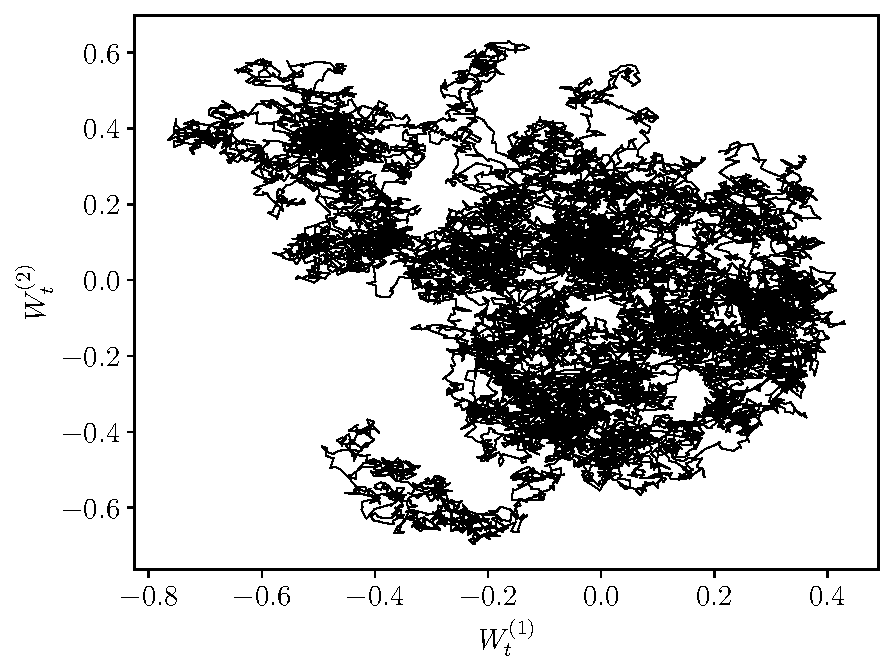
\includegraphics[width=0.49\textwidth]{figures/wiener_realisations_2d.pdf}
		\caption{(Left) Several realisations of a one-dimensional Wiener process \(W_t\) evolving through time, and (right) a realisation of two-dimensional Wiener process \(\left(W_t^{(1)}, W_t^{(2)}\right)\).}
		\label{fig:wiener_rels}
	\end{center}
\end{figure}


\subsection{The It\^o integral}\label{sec:bkg_ito}
\td{Some sort of motivation or introduction}
For our purposes, we can think of an It\^o integral as being defined as the limit in probability of a sequence of sums, i.e. for a scalar but possibly random-valued function \(f\colon [a,b] \to \R\),
\begin{equation}\label{eqn:ito_int_limit_defn}
	\sum_{\left[t_i, t_{i+1}\right] \in \mathcal{P}_N}{f\left(t_{i}\right)\left(W_{t_{i+1}} - W_{t_i}\right)} \xlongrightarrow[\text{probability}]{} \int_a^b{f(t)\dif W_t}, \quad \text{as } N \to \infty
\end{equation}
where \(\mathcal{P}_N\) is a partition of \(\left[a,b\right]\) with \(\lim_{N \to \infty}\mathcal{P}_N = [a,b]\), \emph{\`a la} the definition of the Riemann integral.
It can be shown (see the textbooks by \citet{KallianpurSundar_2014_StochasticAnalysisDiffusion} and \citet{Oksendal_2003_StochasticDifferentialEquations}, for instance) that this limit exists for a large class of both deterministic- and random-valued functions, by constructing appropriate approximations of the function \(f\).

The extension of the It\^o integral to vector- and matrix-valued functions is straightforward.
Let \(g \colon [a,b] \to \R^{n \times m}\) be a function giving possibly random \(n \times m\) matrices (take \(m = 1\) to describe a vector-valued function).
\begin{subequations}\label{eqn:mv_ito_defn}
	Then, we define the It\^o integral of \(g\) with respect to the \(m\)-dimensional Wiener process \(W_t\) over the time interval \([a,b]\) as
	\begin{equation}\label{eqn:mv_ito_defn_1}
		\int_a^b{g(t)\dif W_t} \coloneqq \left(\mathcal{I}_1, \dotsc, \mathcal{I}_n\right)^{\T},
	\end{equation}
	where
	\begin{equation}\label{eqn:mv_ito_defn_2}
		\mathcal{I}_{i} = \sum_{j=1}^m{\int_a^b{g_{ij}\left(t\right) \dif W_t^{(j)}}},
	\end{equation}
	for \(i = 1,\dotsc, n\) and where \(g_{ij}\) denotes the \((i,j)\)th element of \(g\).
\end{subequations}


\subsection{It\^o stochastic differential equations}\label{sec:bkg_sde}

The differential form of an \(n\)-dimensional It\^o stochastic differential equation is
\begin{equation}
	\dif y_t = u\!\left(y_t, t\right)\dif t + \sigma\!\left(y_t, t\right)\dif W_t,
	\label{eqn:gen_sde}
\end{equation}
where the solution \(y_t\) is a stochastic process taking values in \(\R^n\), \(u\colon \R^n \times \R \to \R^n\) is the drift and \(\sigma\colon \R^n \times \R \to \R^{n\times m}\) is the diffusivity.
The driving process \(W_t\) is the \(m\)-dimensional Wiener process.
The notation in \eqref{eqn:gen_sde} is not rigorously defined (the solution \(y_t\) is not differentiable in general, for example), but rather taken as equivalent to the integral form
\begin{equation}
	y_t = y_0 + \int_0^t{u\left(y_\tau, \tau\right)\dif\tau} + \int_0^t{\sigma\left(y_\tau, \tau\right)\dif W_\tau}.
	\label{eqn:gen_sde_int}
\end{equation}
where \(y_0\) is the possibly random initial condition.
In the most general case, the drift \(u\) and diffusivity \(\sigma\) are permitted to themselves be random functions\footnote{For more information, see for instance \citet{KallianpurSundar_2014_StochasticAnalysisDiffusion}.
	The formal treatment of such stochastic differential equations remains an area of open research, such as establishing the conditions for existence and uniqueness of solutions \citehere, and EXAMPLE.}, but in this thesis we assume that both are deterministic.

Stochastic differential equations also arise as the limit of deterministic slow-fast systems, where the average behaviour of the `fast' dynamics can be shown to converge to the solution of a stochastic differential equation \citep[e.g.]{WongZakai_1965_ConvergenceOrdinaryIntegrals,MelbourneStuart_2011_NoteDiffusionLimits,GottwaldMelbourne_2013_HomogenizationDeterministicMaps}\lb{Maybe some better citations out there.}.
A review of this theory is provided by \citet{GivonEtAl_2004_ExtractingMacroscopicDynamics}.
This is particular relevant in climate and physics applications, where \citep{FranzkeEtAl_2015_StochasticClimateTheory}.
This leads to stochastic parameterisation \citep{BernerEtAl_2017_StochasticParameterizationNew,Palmer_2019_StochasticWeatherClimate}, which we review in more detail in \Cref{sec:stoch_param}.




\subsection{Numerical schemes for approximating SDEs}
In general, solving a stochastic differential equation analytically is not possible, and so as with ordinary differential equations we instead look to use numerical schemes to approximate solutions.
However, the solution to a stochastic differential equation is itself a random variable, so a single sample path is not sufficient.
Instead, a numerical SDE scheme produces approximate \emph{realisations} of the solution.
The Euler-Maruyama (EM) method is analogous to the Euler method for ODEs, and considered by many to be the simplest method for numerically solving SDEs \citep{KloedenPlaten_1992_NumericalSolutionStochastic}.
The update step of the EM scheme, with step size \(\Delta t\), is
\begin{equation}
	\hat{x}_{t + \Delta t} = \hat{x}_{t} + \Delta t u\left(\hat{x}_t, t\right) + \Delta t \sigma\left(\hat{x}_t, t\right) Z_t,
	\label{eqn:em_step}
\end{equation}
where \(Z_t\) is sampled from the standard Gaussian \(\Gauss{0,I}\), and the scheme is initialised as \(\hat{x}_0 = x_0\).
The Euler-Maruyama scheme has strong order 0.5, meaning that
\[
	\avg{\norm{x_t - \hat{x}_{t}\left(\Delta t\right)}} = \mathcal{O}\left(\Delta t^{0.5}\right),
\]
where \(\hat{x}_t\left(\Delta t\right)\) is the Euler-Maruyama estimate at time \(t\) using step size \(\Delta t\).


There are many other schemes for generating approximate samples of a stochastic differential equation, of varying weak and strong orders.
For instance, extensions of Runge-Kutta-type schemes \citep{Roberts_2012_ModifyImprovedEuler,Rossler_2010_RungeKuttaMethodsStrong}.






\subsection{The Fokker-Planck equation}\label{sec:fp_eqn}
The probability density function \(\rho: \R^n \times [0,T] \to [0,\infty)\) for the solution to \eqref{eqn:gen_sde} at time \(t \in [0,T]\) is the solution to the corresponding Fokker-Planck equation \citep{Risken_2012_FokkerPlanckEquationMethods}
\begin{equation}
	\dpd{\rho}{t} = \frac12\nabla\cdot\nabla\cdot\left(\rho\sigma\sigma^{\T}\right) - \nabla\cdot\left(\rho u\right)
	\label{eqn:fp_eqn}
\end{equation}
subject to some initial density \(\rho\left(x,0\right)\) given by the initial condition to \eqref{eqn:gen_sde}.
To ensure that the solution is a valid probability density function on \(\R^n\), for any \(t \in [0,T]\), \(\rho\) must satisfy
\begin{subequations}\label{eqn:fp_valid_pdf}
	\begin{align}
		\int_{\R^n}{\rho\left(x, t\right)\dif x} = 1, \label{eqn:fp_valid_pdf_norm} \\
		\lim_{x \to \infty}\rho\left(x,t\right) = 0. \label{eqn:fp_valid_pdf_limit}
	\end{align}
\end{subequations}
For a fixed and deterministic initial condition \(y_0 = x\), the corresponding initial condition to \eqref{eqn:fp_eqn} is the Dirac-delta distribution centred at \(x\).


\subsubsection{Relationship to the classical advection-diffusion equation}
The advection-diffusion equation describes the time-evolution of a passive and inert scalar quantity, such as temperature, salinity

\citep{Visser_2008_LagrangianModellingPlankton}

Let \(c \colon \Omega_0 \times [0,T] \to [0, \infty)\) denote the concentration of a passive and inert scalar quantity, then the classical advection-diffusion equation is
\begin{equation}\label{eqn:advec_diff}
	\dpd{c}{t} = - \nabla\cdot \left(v\!\left(x,t\right)c\!\left(x,t\right)\right) + \nabla\cdot\left(K\!\left(x,t\right)\nabla c\!\left(x,t\right)\right), \quad c\!\left(x,0\right) = c_0\!\left(x\right),
\end{equation}
where \(v\) denotes the flow velocity dictating the advection (displacement) of the tracer, and \(K\) is a matrix describing the diffusion (dispersion) of \(c\).




If we set \(u\!\left(x,t\right) = v\!\left(x,t\right) + \nabla \cdot K\!\left(x,t\right)\) and \(\sigma\!\left(x,t\right)\sigma\!\left(x,t\right) = K\!\left(x,t\right)\), then the Fokker-Planck equation \cref{eqn:fp_eqn} is equivalent to the advection-diffusion equation \eqref{eqn:advec_diff}.
Thus, the evolution of the tracer concentration under \cref{eqn:advec_diff} can be equivalently considered as the probability density function of solutions to the stochastic differential equation
\begin{equation}\label{eqn:ad_sde}
	\dif x_t = \left[u\!\left(x_t, t\right) + \nabla \cdot K\!\left(x_t, t\right)\right]\dif t + \kappa\!\left(x_t, t\right)\dif W_t, \quad x_t \sim \hat{c}_0,
\end{equation}
where \(\kappa\) is any matrix-valued function satisfying \(K \equiv \kappa\kappa^{\T}\), and
\[
	\hat{c}_0\!\left(x\right) = \frac{c_0\!\left(x\right)}{\int_{\Omega_0}c_0\!\left(z\right)\dif z},
\]
is the initial density of \eqref{eqn:advec_diff} normalised to describe a probability density function.
Assuming that the total concentration tracer is conserved, that is
\[
	\int_{\Omega_t}{c\!\left(z,t\right)\dif z} = \int_{\Omega_0}{c_0\!\left(z\right)\dif t}
\]
for all \(t \in [0,T]\), then we can recover \(c\) from the probability density function \(\rho\) corresponding to \cref{eqn:ad_sde} as
\[
	c\!\left(x,t\right) = \rho\!\left(x,t\right)\int_{\Omega_0}{c_0\!\left(z\right)\dif t}.
\]
An implication of this connection is that the theory and computations for stochastic differential equations developed throughout this thesis can be applied to \emph{any} scalar field that is modelled with an advection-diffusion type equation.



\subsubsection{Practical difficulties}

However, there are several practical difficulties with using the Fokker-Planck equation:
\begin{itemize}
	\item \textbf{Dimensionality:}
	\item \textbf{Boundary conditions:}
\end{itemize}



\subsubsection{Green's function method}
The Fokker-Planck equation is linear, so we can apply a technique known as Green's function method (for an example of this approach on a linear SDE, see Section 3.2 of \citet{Risken_2012_FokkerPlanckEquationMethods}) in order to understand the behaviour of solutions with non-fixed initial conditions.
Let \(\mathcal{P}_t\set{\rho_0}\) denote the solution operator of \eqref{eqn:fp_eqn} with initial density \(\rho_0\colon \R^n \to \R^n\).
Then, since \eqref{eqn:fp_eqn} is a linear equation, \(\mathcal{P}_t\) is a linear operator.
Now, let \(x_0 \in \R^n\) be an arbitrary fixed point, and consider the fundamental solution, or Green's function,
\[
	G_t\left(x; x_0\right) \coloneqq \mathcal{P}_t\set{\delta_{x_0}}\!\left(x\right).
\]
That is, \(G_t\left(x; x_0\right)\) is the solution to the Fokker-Planck equation with the Dirac-delta initial condition \(\delta_{x_0}(x) = \delta\left(x - x_0\right)\), which is equivalent to the SDE \eqref{eqn:gen_sde} with the deterministic and fixed initial condition \(y_0 = x_0\).
The Green's function \(G_t\) is equivalently the transition probability function of the SDE solution \(x_t\) as a stochastic process.
Now, using the sampling property of the Dirac-delta function, for a general initial density \(\rho_0\colon \R^n \to \R^n\),
\[
	\rho_0(x_0) = \int_{\R^n}{\rho_0\left(x\right)\delta_{x_0}\left(x\right)\dif x}.
\]
Since \(\mathcal{P}_t\) is linear,
\begin{equation}
	\mathcal{P}_t\set{\rho_0}\!\left(x_0\right) = \int_{\R^n}{\rho_0\!\left(x\right)\mathcal{P}_t\set{\delta_{x_0}}\!\left(x\right)\dif x} = \int_{\R^n}{\rho_0\!\left(x\right) G_t\!\left(x; x_0\right)\dif x}.
	\label{eqn:fp_greens_trick}
\end{equation}



\section{Stochastic parameterisation}\label{sec:stoch_param}

Many numerical weather and climate prediction models rely upon a spatial discretisation for tractable analysis and simulation.
Often, an extremely high resolution is needed to produce accurate simulations and predictions; for example, \citet{DawsonEtAl_2012_SimulatingRegimeStructures} demonstrated such requirements\lb{Read paper and be specific about numbers} for the state-of-the-art European Centre for Medium-Range Weather Forecasts (ECMWF) forecast model.

The formal introduction of stochastic terms to account for unknown and unresolved processes into an otherwise deterministic model is known as \emph{stochastic parameterisation}, particularly in scientific circles.
\citet{BernerEtAl_2017_StochasticParameterizationNew} review the need for stochastic parameterisation in weather and climate models and discuss how stochastic terms can quantify four different aspects of these models:
\begin{itemize}
	\item directly estimating uncertainty,
	\item reducing systematic model errors arising from unresolved subgrid processes,
	\item triggering regime changes, and
	\item encapsulating the effect of external forcing.
\end{itemize}


\begin{figure}
	\begin{center}
		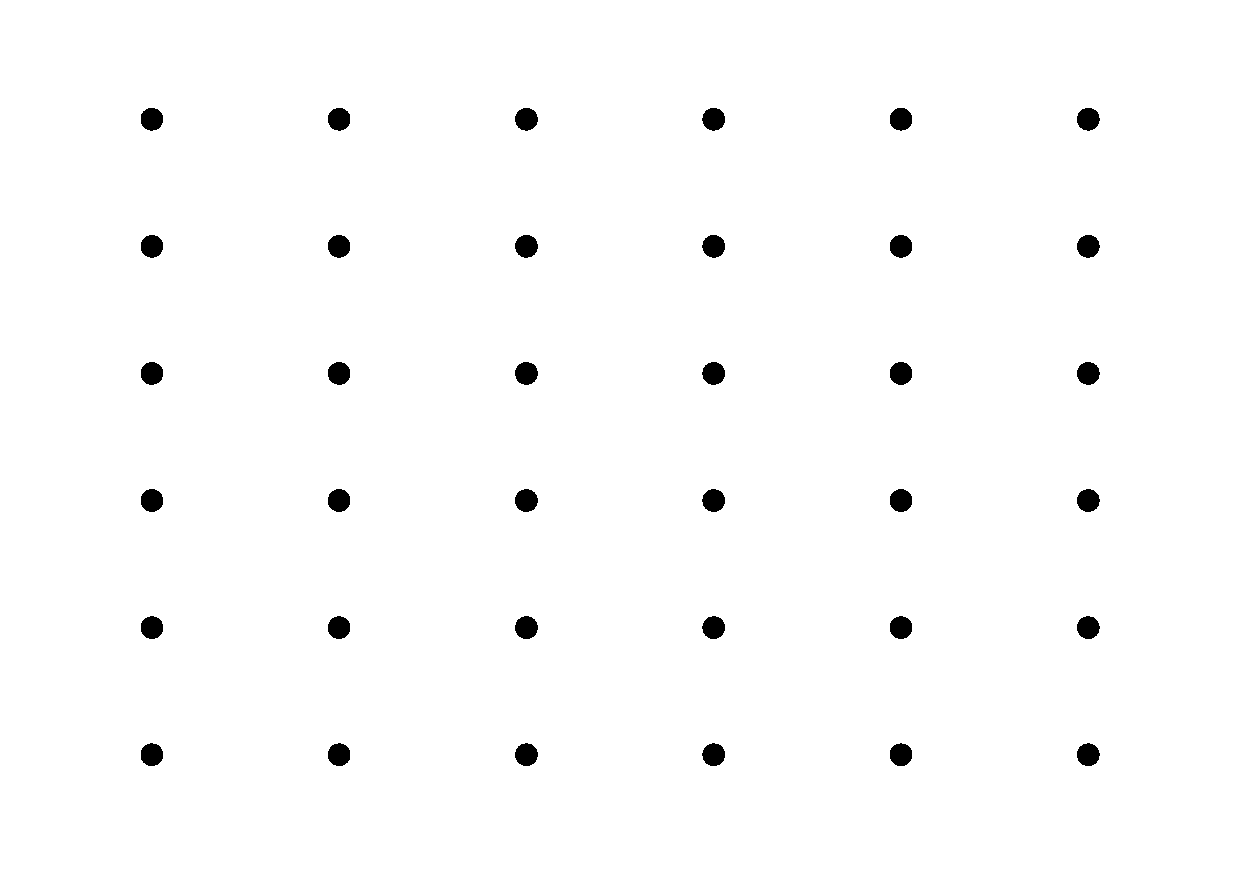
\includegraphics[width=\textwidth]{chp02_background/figures/gridpoints.pdf}
		\caption{An illustration of unresolved subgrid effects in a spatial discretisation.
			When a system is discretised, either from measurements or to numerically solve a model, processes between the grid points and no longer resolved or observed and yet can have a noticeable impact on the system.}
		\label{fig:subgrid_effects}
	\end{center}
\end{figure}


In particular, \citet{SuraEtAl_2005_MultiplicativeNoiseNonGaussianity} demonstrate that linear deterministic dynamics with multiplicative noise can be produce the non-Gaussian statistics that we observed in real systems.

\citet{DawsonPalmer_2015_SimulatingWeatherRegimes} showed through simulation studies that the performance of a high-resolution purely deterministic model can be matched by a lower-resolution stochastic model.


The mathematical formulation of stochastic parameterisation -- where model predictions are now random quantities -- lends itself naturally to data assimilation \citep{BudhirajaEtAl_2019_AssimilatingDataModels,Jazwinski_2014_StochasticProcessesFiltering,LawEtAl_2015_DataAssimilationMathematical,ReichCotter_2015_ProbabilisticForecastingBayesian}, where ongoing observations are combined with predictions from a model to produce an improved forecast.
Data assimilation provides a framework that can simultaneously account for uncertainty in the observations and the model itself.
It has been shown that stochastic parameterisation can improve the quality of forecasts in data assimilation schemes \citep{MitchellGottwald_2012_DataAssimilationSlow,HaEtAl_2015_ComparisonModelError}, and so these applications are an active error of research \citep[e.g.]{GottwaldHarlim_2013_RoleAdditiveMultiplicative}.

\td{Flow from here into the need for maths - justifications, proofs, etc.?}
There is an emerging need to bridge the gap between mathematicians working on developing stochastic theory and algorithms, and the scientists looking to apply this work to their respective fields.
In particular, \citet{BernerEtAl_2017_StochasticParameterizationNew} conclude that ``geoscientists are often unaware of mathematically rigorous results that can aid in the development of physically relevant parameterizations, [while] mathematicians often do not know about open issues in scientific applications that might be mathematically tractable''.


Although stochastic parameterisation is more common in the atmospheric modelling context, oceanography also suffers from the same trade-off between spatial resolution and accuracy of predictions.

In the context of a fluid, unresolved processes can be vortices, eddies and turbulence \citep{Griffa_1996_ApplicationsStochasticParticle}.

The mixing effect that these eddies have on the surrounding flow can be modelled with spatiotemporally-varying diffusion \citehere, which via the Fokker-Planck equation can be equivalently formulated as a stochastic differential equation with multiplicative noise.
The Lagrangian trajectories, incorporating these unresolved eddy effects, are then modelled as solutions to the stochastic differential equation.
Equivalently, through the Fokker-Planck equation we can consider the evolution of a passive tracer undergoing advection due to the deterministic drift and diffusion from both any natural diffusivity and the unresolved processes.
The probability density function that solves the Fokker-Planck equation can be instead thought of as a time-varying density (with the appropriate normalisation) of the tracer.
For instance, the Fokker-Planck equation has been used to model the transport of ??? with a stochastic framework \citehere.
Hence, understanding the evolution of solutions to a stochastic differential equation is valuable in oceanography, as a means of quantifying both observational error and unresolved subgrid processes.


There are several different methods for quantifying eddy diffusivity given either observed tracer data or a global ocean circulation model.

The simplest notion of eddy diffusivity is a defined by






A recent approach by \cite{YingEtAl_2019_BayesianInferenceOcean} uses Bayesian inference to estimate the eddy diffusivity tensor from observed Lagrangian tracer data, by numerically solving the Fokker-Planck equation to compute a likelihood function.


In summary, stochastic parameterisation



\section{Limitations of stochastic simulation and the need for further development}\label{sec:bkg_sim_limits}
The introduction of stochastic terms complicates both the analytical treatment of the model.
For example, we saw in \Cref{sec:sde_theory} that adding even additive and stationary\lb{Is this the right word?? I mean that \(\sigma\) is constant, with no time-dependency}\td{need to define additive versus multiplicative properly.} noise to an analytically solvable non-linear deterministic model can make exact solutions intractable.
Thus, across many applications the state of the art approach is to generate samples of the stochastic model and perform statistical inference.
For example, Monte-Carlo simulation is used across weather forecasting \citep{LeutbecherEtAl_2017_StochasticRepresentationsModel}, \td{something atmospheric} and \td{something oceanic}.

However, the most significant drawback of bulk stochastic simulation is the computational load.
In general, a large number of samples is required for convergent statistics and accurate inference, as discussed by \citet{Leutbecher_2019_EnsembleSizeHow}.
For a complex model, the computational load of computing a single realisation

The recent review by \citet{LeutbecherEtAl_2017_StochasticRepresentationsModel} highlights the need to develop computationally efficient schemes for quantifying stochasticity in weather and climate forecast models.


\td{Show the plateauing out that I am observing empirically when using a KDE . . . some literature on this?? This is a huge point to make}
For example, suppose that we intend on using the probabilistic forecast of our stochastic model in an inference scheme, such as in data assimilation in which model predictions are combined with ongoing observations to produce an improved forecast \cite[e.g.]{LawEtAl_2015_DataAssimilationMathematical,BudhirajaEtAl_2019_AssimilatingDataModels, ReichCotter_2015_ProbabilisticForecastingBayesian}.
This requires a probability density function or similar for our forecast, but in generating samples we initially only have a collection of finite discrete points.


The overall aim of this thesis is to address this problem, by developing characterisations of uncertainty and algorithms for approximating solution probability densities (as opposed to just generating samples) that are computationally efficient.
We aim to take advantage of the computational ease of generating solutions to a deterministic system (relative to taking many samples of a stochastic one).


The purpose of this example was to highlight the importance of accounting for measurement error and unresolved processes in a ; when the dynamics are complicated, then any uncertainty can have a significant impact on our inferences from the model, both quantitatively and qualitatively.



\section{Stochastic sensitivity}\label{sec:s2_summ}
To conclude our background and motivation, this section provides a brief summary of stochastic sensitivity, as introduced by \citet{Balasuriya_2020_StochasticSensitivityComputable} as a means of quantifying uncertainty
Further technical details, including the main theorems, are reproduced in \Cref{app:s2_details}.

Given possibly time-dependent velocity data \(u: \R^2 \times [0,T] \to \R^2\), \citet{Balasuriya_2020_StochasticSensitivityComputable} considers the evolution of solutions to the differential equation
\[
	\dod{x_t}{t} = u\left(x_t, t\right).
\]
Solutions can be summarised by the flow map \(F_{t_1}^{t_2}\), as in \Cref{def:flow_map}.
In most practical situations, the Eulerian velocity data driving ocean and atmospheric models relies upon measurements of estimates obtained on a low resolution spatial discretisation.
\citet{Balasuriya_2020_StochasticSensitivityComputable} introduces stochastic sensitivity as a new tool for directly quantifying the impact of Eulerian uncertainty on Lagrangian trajectories.
The evolution of Lagrangian trajectories is modelled as solution to a It\^o stochastic ordinary differential equation.

To directly account for these unresolved sources of uncertainty, the ``true'' Lagrangian trajectories evolve as solution to the stochastic differential equation
\begin{equation}
	\sde{y_t}{u\left(y_t, t\right)}{\epsilon\sigma\left(y_t, t\right)},
	\label{eqn:ss_sde},
\end{equation}
where \(0 < \epsilon \ll 1\) is a parameter quantifying the scale of the noise, \(\sigma:	\R^2\times[0,T] \to \R^{2\times 2}\) is the \(2\times 2\) diffusion matrix, and \(W_t\) is the canonical two-dimensional Wiener process.
In the original formulation \citep{Balasuriya_2020_StochasticSensitivityComputable}, \(\epsilon\) is a dimensionless parameter and \(\sigma\) is dimensional, but an alternative scaling technique relates \(\epsilon\) to spatial and velocity uncertainty scales in the data (see the follow-up work by \citet{BadzaEtAl_2023_HowSensitiveAre,Balasuriya_2020_UncertaintyFinitetimeLyapunov,FangEtAl_2020_DisentanglingResolutionPrecision})
Since \(\sigma\) can vary by both space and time, the noise is multiplicative.
The diffusion matrix \(\sigma\) is specified \emph{a priori}, based on any knowledge of how uncertainty varies with space and time, e.g. from experimental considerations, observation error estimates.
If no such prior information is known, then \(\sigma \equiv I\), the \(2 \times 2\) identity matrix is the default choice.

To quantify uncertainty in a way that is independent of the noise scale \(\epsilon\), \citet{Balasuriya_2020_StochasticSensitivityComputable} defined the random variable \(z_\epsilon\left(x,t\right)\) on \(\R^2 \times [0,T]\) as
\[
	z_\epsilon\left(x,t\right) \coloneqq \frac{y_t - F_0^t(x)}{\epsilon}.
\]
The main aim is to compute statistics of \(z_\epsilon\) at the final time \(T\), so that of \(z_\epsilon\left(x,T\right)\).
\citet{Balasuriya_2020_StochasticSensitivityComputable} then considers the signed projection of \(z_\epsilon\left(x,T\right)\) onto a ray emanating from the deterministic position \(F_0^T(x)\) in a given direction, defining
\[
	P_\epsilon\left(x,\theta\right) \coloneqq \hat{n}^{\T} z_\epsilon(x,T),
\]
where \(\theta \in \left[-\pi/2, \pi/2\right)\) and
\[
	\hat{n}(\theta) = \begin{bmatrix}
		\cos{\theta} \\
		\sin{\theta}
	\end{bmatrix}.
\]

The statistics of \(z_\epsilon\left(x,T\right)\) and \(P_\epsilon(x,\theta)\) are considered in the limit as \(\epsilon\downarrow 0\), which provides a characterisation of the uncertainty of the model \emph{independently} of the scale of the noise.
\citet{Balasuriya_2020_StochasticSensitivityComputable} provided computable expressions for the mean and variance of \(P_\epsilon\left(x,\theta\right)\) in this limit of small noise, which we summarise here.
For proofs of these results, see the appendices of \citet{Balasuriya_2020_StochasticSensitivityComputable}.

\begin{definition}[\citealt{Balasuriya_2020_StochasticSensitivityComputable}]
	\begin{alpharate}
		\item The \textbf{anisotropic uncertainty} is a scalar field \(A: \R^2\times\left[-\pi/2, \pi/2\right) \to [0,\infty)\) defined by
		\[
			A(x,\theta) \coloneqq \sqrt{\lim_{\epsilon\downarrow 0}\var{P_\epsilon(x,\theta)}}.
		\]

		\item The \textbf{stochastic sensitivity} is a scalar field \(S: \R^2 \to [0,\infty)\) defined by
		\[
			S^2(x) \coloneqq \lim_{\epsilon\downarrow 0}\sup_{\theta}{\var{P_\epsilon(x,\theta)}}.
		\]
	\end{alpharate}
\end{definition}

By employing techniques from both deterministic and stochastic calculus (i.e. Gr\"onwall's inequality, the Burkholder-Davis-Gundy inequality, It\^o's Lemma), Balasuriya further established expressions for both the anisotropic uncertainty and the stochastic sensitivity that are computable given only the flow map and velocity data.

\begin{theorem}[\citealt{Balasuriya_2020_StochasticSensitivityComputable}]\label{thm:orig_s2_calculation}
	For \(x \in \R^2\), set \(w \coloneqq F_0^t(x)\).
	Then, for any \(\theta \in \left[-\pi/2, \pi/2\right)\),
	\[
		A(x,\theta) = \left(\int_0^T{\norm{\Lambda\left(x, t, T\right)J\hat{n}(\theta)}\dif t}\right)^{1/2},
	\]
	where
	\[
		\Lambda\left(x,t,T\right) \coloneqq e^{\int_t^T{\left[\nabla \cdot u\right]\left(F_0^\xi(x), \xi\right)\dif\xi}}\sigma\left(F_0^t(x), t\right)^{\T}J \nabla_w F_T^t\left(w\right),
	\]
	with the gradients \(\nabla_w\) of the flow map taken with respect to the mapped position \(w\), and
	\[
		J \coloneqq \begin{bmatrix}
			0 & -1 \\
			1 & 0
		\end{bmatrix}
	\]
	Additionally, stochastic sensitivity is computed as
	\[
		S^2(x) = P(x) + N(x),
	\]
	with
	\begin{align*}
		L(x) & \coloneqq \frac12\sum_{i=1}^2\int_0^T\left[\Lambda_{i2}\left(x,t, T\right)^2 - \Lambda_{i1}\left(x,t,T\right)^2\right]\dif t \\
		M(x) & \coloneqq \sum_{i=1}^2\int_0^T{\Lambda_{i1}\left(x,t,T\right)\Lambda_{i2}\left(x,t,T\right)\dif t}                           \\
		N(x) & \coloneqq \sqrt{L^2(x) + M^2(x)}                                                                                             \\
		P(x) & \coloneqq \abs{\frac12\sum_{i=1}^2\sum_{j=1}^2{\int_0^T{\Lambda_{ij}\left(x,t,T\right)^2\dif t}}},
	\end{align*}
	where \(\Lambda_{ij}\) is the \((i,j)\)-element of \(\Lambda\).
\end{theorem}





\subsection{Current applications \& shortcomings}
Since stochastic sensitivity is only a recent development, it has only been applied in a limited number of places so far.
Here, we briefly review the literature in which the original formulation stochastic sensitivity by \citet{Balasuriya_2020_StochasticSensitivityComputable} has been applied.

\begin{itemize}
	\item \citet{Balasuriya_2020_UncertaintyFinitetimeLyapunov} uses stochastic sensitivity to compute an error bound for the finite-time Lyapunov (FTLE) computation.
	      The computable \(S^2\) value is used as an estimate of the standard deviation of the deviation between the deterministic and ``true'' (stochastic) trajectories, leading to a computable error bound on the FTLE value.


	\item \citet{FangEtAl_2020_DisentanglingResolutionPrecision}


	\item \citet{BadzaEtAl_2023_HowSensitiveAre} investigate the impact of velocity uncertainty on Lagrangian coherent structures (e.g. see the reviews by \citet{BalasuriyaEtAl_2018_GeneralizedLagrangianCoherent} and \citet{HadjighasemEtAl_2017_CriticalComparisonLagrangian}) extracted as robust sets with stochastic sensitivity.
	      The stochastic model \cref{eqn:ss_sde} is used to generate realisations of Lagrangian trajectories subject to noise on the velocity field.
	      By directly capturing such uncertainty as a means of coherent set \citet{BadzaEtAl_2023_HowSensitiveAre} showed that robust sets extracted with stochastic sensitivity do SOMETHING.

\end{itemize}
There are several limitations to the work as originally presented by \citet{Balasuriya_2020_StochasticSensitivityComputable}:
\begin{enumerate}
	\item The tools are restricted to two-dimensional models, and the constructions using projections have no obvious extension to \(n\)-dimensions.
	      Extending stochastic sensitivity to \(n\)-dimensions will enable application to a much broader class of models beyond the fluid flow context, including high-dimensional climate models.

	\item \citet{Balasuriya_2020_StochasticSensitivityComputable} only computes the expectation and variance of the projections \(P_\epsilon(x,\theta)\), which does not give us the distribution under the limit as \(\epsilon\) approaches 0.

	\item The computational formula for the anisotropic uncertainty and stochastic sensitivity, as described in \Cref{thm:orig_s2_calculation}, require knowledge of the divergence \(\nabla\cdot u\) of the velocity field, and computation of four integrals.
\end{enumerate}



In \Cref{sec:theory_s2}, we present an extension of stochastic sensitivity to \(n\)-dimensions that overcomes these limitations.
